\subsection{View names and weak-target summaries}
\inputtable{tab13_views}


\paragraph{Additional weak-target summaries.}
On test, full VCRE-Fib has mean inside attention 0.570815, outside response fraction 0.666595, and inside/outside mean-response ratio 359,012.493654; w/o View has 0.499237, 0.550558, and 1,678,411.504391, respectively. The outside response fraction is the summed attention outside the target boxes divided by total attention. The last ratio clips its denominator at $10^{-8}$, so full-field boxes can yield very large values. These are descriptive response summaries, not localization-accuracy measures. Table~\ref{tab:views} compares class recall for the two view-capable models; evaluation artifacts also provide prediction frequencies and confusion matrices.

\subsection{Case selection and display protocol}\label{sec:appendix-case-protocol}
View metrics include accuracy/macro-F1; weak-target Dice/IoU use threshold 0.5. From pools of 12 test and four validation cases, four full-model test cases spanning four true views were selected for the main figure and two validation cases for the appendix. Correspondence candidates were prioritized by weak-box Dice within view. Expansion candidates required an outside response fraction of 0.5--0.9 (summed attention outside the target boxes divided by total attention), Dice above 0.1, a thresholded response intersecting the boxes, and at least 10\% of its area outside all displayed boxes. Patients were deduplicated within each pool. All panels use the same processed ROI, fixed $[0,1]$ localization scale, opacity 0.55, and cyan 0.5 contour. These are selected illustrations; clinical descriptions of the extended regions are not assigned.

The main paper presents four selected test cases. Figure~\ref{fig:valcases} shows two selected validation examples with responses extending beyond local boxes. These examples are separate from the test ranking and spatial metrics; the first also shows a disagreement between the reference and predicted views.
\begin{figure}[!htbp]
\centering
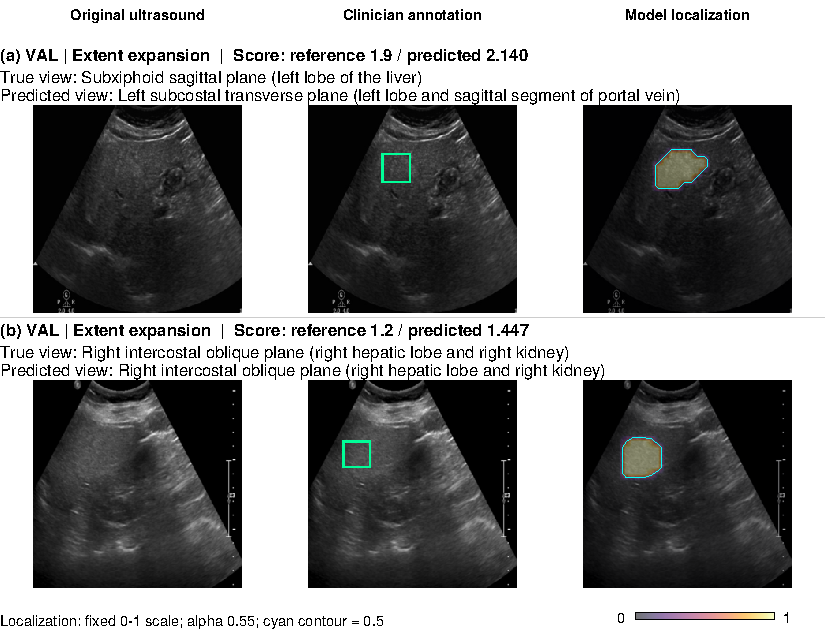
\includegraphics[width=\linewidth]{figures/assets/fig06_validation_cases.pdf}
\caption{Selected validation examples with responses beyond local boxes. Predictions use the frozen checkpoint evaluated quantitatively. The three columns show the original ROI, clinician annotation, and model localization; labels report reference and predicted scores and acquisition views. In the first example, the predicted view differs from the reference. Responses beyond local boxes identify locations for inspection, without establishing complete lesion extent.}
\label{fig:valcases}
\end{figure}
